\documentclass[11pt]{article}
\usepackage{amsmath}
\usepackage{mathtools}
\usepackage{amssymb}
\usepackage{hyperref}
\usepackage{graphicx}
\usepackage{listings}
\lstset{
  basicstyle=\ttfamily,
  mathescape
}
\setlength{\parskip}{5pt}

\begin{document}
\title{NES}
\author{Carmine Marra, Stefano Mercogliano, Daniele Ottaviano, Francesco Vitale}
\date{}
\maketitle
\tableofcontents
\clearpage
\section{Descrizione del processo}

\section{Avvio}
\subsection{Vision}
Si vuol sviluppare un sistema, definito NES, che sia comprensivo di \emph{emulatore} e \emph{assemblatore}. L'assemblatore consentirà agli utenti del sistema di poter assemblare il proprio programma, scritto ovviamente secondo il modello di programmazione del processore di riferimento, e, consecutivamente, caricare questo programma nell'emulatore consentendo l'esecuzione di quest'ultimo.\\
L'utente deve poter essere in grado di poter scrivere il proprio programma, interagire con l'assemblatore e assemblare il proprio programma secondo le opzioni messe a disposizione dal sistema stesso; l'utente potrà specificare qualsiasi elemento sintattico appartenente all'ISA del NES: l'assemblatore sarà in grado di interpretare quanto viene specificato dal programma e tradurre il codice e predisporlo per l'esecuzione sull'emulatore.\\
D'altro canto l'utente può decidere di caricare qualsiasi programma assembler sull'emulatore, che sia il programma assemblato con l'assemblatore del sistema, oppure no. L'emulatore non è finalizzato solo all'esecuzione delle linee di codice, ma è destinato anche alla visualizzazione grafica di alcune proprietà interne della macchina emulata durante l'esecuzione del programma, come:
\begin{itemize}
	\item{
		Il comportamento del processore e dei suoi registri interni;
	}
	\item{
		La memoria RAM in qualsiasi range di indirizzi;
	}
	\item{
		Informazioni al contorno;
	}
	\item{
		Il comportamento della PPU e il rendering grafico;
	}
	\item{
		Il comportamento interno della APU;
	}
\end{itemize}
\clearpage
\subsection{Specifiche supplementari}
L'architettura deve essere modulare, soprattutto in vista di un completo disaccoppiamento dell'emulatore dall'assemblatore: l'emulatore dev'essere in grado di poter caricare qualsiasi sorgente assemblato da qualsiasi altro assemblatore, a patto che l'estensione sia la stessa.\\
Essendo che assemblatore ed emulatore saranno completamente disaccoppiati, il sistema risulterà essere \emph{robusto}; l'assemblatore, quindi, sarà un componente \emph{riusabile}, perchè produrrà codice compliant con altri emulatori.\\
In vista di un approccio agile, e quindi incrementale ed evolutivo, \emph{manutenibilità} e \emph{evolvibilità} sono importanti: entrambi i sottosistemi, essendo complessi, si prestano a essere decomposti in moduli idealmente lascamente accoppiati: bisogna assecondare questa proprietà al fine di ottenere uno sviluppo incentrato sulle parti critiche del sistema, per poter poi \emph{estendere} quanto già sviluppato nelle prime iterazioni.\\
Si vuole anche rendere il sistema quanto più \emph{interattivo} possibile: data la natura dell'emulatore, il sistema stesso potrebbe risultare poco \emph{usabile}. Le scelte di design dovranno in qualche modo rendere il sistema più user-friendly.
\subsection{Glossario}
\clearpage

\section{Specifica dei requisiti}
In questa sezione ci riconduciamo ai suggerimenti tratti dal Larman per la stesura dei requisiti funzionali. In particolare, ci concentreremo sulla stesura di artefatti che catturino degli use-case che risultino essere \emph{goal-driven}, ossia incentrandoci sugli obbiettivi degli utenti che sfruttano il sistema.

\subsection{Attori e Obiettivi}
Attori:
\begin{itemize}
	\item{Utente}
\end{itemize}
Obiettivi utente:
\begin{enumerate}
	\item{
		Esegui programma utente (Scegliendolo dalla lista o dal file system)
	}
	\item{
		Gestisci Lista programmi (Carica/ Modifica/ Elimina)
	}
	\item{
		Configura Emulazione (Velocità/Periferica)
	}
	\item{
		Gestione Codice Sorgente (Scrivi/Salva/Carica)
	}
	\item{
		Compila il Codice 
	}
	\item{
		Visualizza Stato Architettura 
	}
\end{enumerate}

Descrizione in breve dei casi d’uso:
\begin{itemize}
\item{
	EseguiProgramma: Il programmatore potrà eseguire il programma ed eventualmente visualizzare a schermo l’esecuzione. L’esecuzione potrà essere fatta sia in modalità standard che istruzione per istruzione.
}
\item{
	CaricaInLista: L’utente carica un programma dal suo computer all’applicazione. Il programma verrà aggiunto alla lista dei programmi eseguibili.
}
\item{
	EliminaDallaLista: L’utente seleziona dalla lista un programma e lo rimuove dalla lista.
}
\item{
	ConfiguraEmulazione: L’utente prima dell’esecuzione di un programma potrà cliccare su di un pulsante per visualizzare e modificare i parametri di emulazione come la Velocità dell’esecuzione, le periferiche di ingresso e di uscita, la grandezza dello schermo etc. 
}
\item{
	CompilaCodice: Permette di compilare il codice scritto producendo un file macchina comprensibile per l’emulatore.
}
\item{
	VisualizzaStatoArchitettura: Il programmatore potrà cliccare sull’immagine di una specifica componente hardware emulata per verificare il comportamento della stessa durante l’esecuzione di un programma
}
\end{itemize}
\subsection{Use-case model}
\begin{table}[h]
\begin{tabular}{|l|l|}
\hline
\textbf{Nome del caso d'uso}      & EseguiProgramma                                                                                                                                                                                                        \\ \hline
\textbf{Portata}                  & User-level                                                                                                                                                                                                             \\ \hline
\textbf{Attore primario}          & Utente                                                                                                                                                                                                                 \\ \hline
\textbf{Stakeholders e interessi} & Selezionare il programma ed eseguirlo                                                                                                                                                                                  \\ \hline
\textbf{Pre-condizioni}           & Modalità d'esecuzione scelta                                                                                                                                                                                                                       \\ \hline
\textbf{Post-condizioni}          & Visualizzazione dell'esecuzione del programma                                                                                                                                                                          \\ \hline
\textbf{Scenario principale}      & \begin{tabular}[c]{@{}l@{}}1. Seleziona programma\\ 2. Avvia programma\end{tabular}                                                                                                                                    \\ \hline
\textbf{Estensioni}               & \begin{tabular}[c]{@{}l@{}}1a. L'utente seleziona il programma dalla lista\\ 1b. L'utente seleziona il programma dal file system\\ 2a. L'utente sospende il programma\\ 2b. L'utente arresta il programma\end{tabular} \\ \hline
\end{tabular}
\end{table}

\begin{table}[h]
\begin{tabular}{|l|l|}
\hline
\textbf{Nome del caso d'uso}      & VisualizzaStatoArchitettura                                                                                                                                                                                                                                                                             \\ \hline
\textbf{Portata}                  & User-level                                                                                                                                                                                                                                                                                              \\ \hline
\textbf{Attore primario}          & Utente                                                                                                                                                                                                                                                                                                  \\ \hline
\textbf{Stakeholders e interessi} & Verificare l'evoluzione dello stato dell'architettura                                                                                                                                                                                                                                                   \\ \hline
\textbf{Pre-condizioni}           & Il programma non è in esecuzione                                                                                                                                                                                                                                                                        \\ \hline
\textbf{Post-condizioni}          & Visualizzazione dello stato dell'architettura                                                                                                                                                                                                                                                           \\ \hline
\textbf{Scenario principale}      & 1. Seleziona componente                                                                                                                                                                                                                                                                                 \\ \hline
\textbf{Estensioni}               & \begin{tabular}[c]{@{}l@{}}1a. Se selezionata la CPU\\ \quad1. Mostra tutti i registri\\ 1b. Se selezionata la memoria\\ \quad 1. Seleziona range\\ \quad 2. Mostra porzione di memoria\\ 1c. Se selezionata la PPU\\ 1d. Se selezionata la APU\end{tabular} \\ \hline
\end{tabular}
\end{table}
\subsection{Feature list}

\subsubsection{Rendering grafico}
All'utente è concessa la possibilità di poter caricare le cosiddette \emph{cartucce}, delle ROM scritte in linguaggio assembly adoperando il modello di programmazione offerto dall'architettura del NES, ossia la macchina che sta venendo emulata.\\
Poichè il rendering grafico è impossibile senza che venga emulata una componente molto importante della architettura, ossia la PPU, è necessario esplorare in dettaglio questo importante componente, e le memorie con cui esso comunica.

La Picture Processing Unit (PPU) è vista dalla CPU montata dal NES come un dispositivo I/O; infatti, la comunicazione con questa unità avviene mediante dei registri (trattasi di \emph{memory-mapped I/O}). La PPU può però essere pienamente classificata come un'unità di elaborazione molto complessa, probabilmente, dal punto di vista implementativo, ancor più della CPU.\\
Essa è ovviamente una macchina sequenziale, che evolve in diversi stati; il suo obbiettivo è quello di \emph{renderizzare}, ossia \emph{disegnare} a schermo, i vari pixel che derivano dalle memorie attaccate alla PPU, ma anche interne alla cartridge. Detto ciò, analizziamo il sottosistema d'interesse:
\begin{figure}[h]
\centering
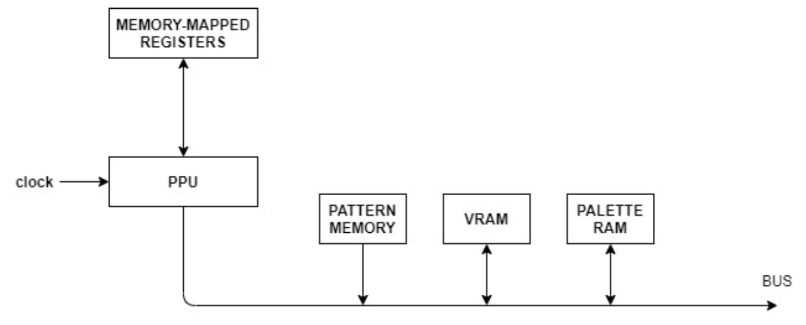
\includegraphics[width=400px, height=156px]{PPUARCH.jpg}
\end{figure}\\
Come si vede, a connettere la PPU è un BUS, che consente il colloquio della PPU con le memorie che sono ad essa fisicamente (e logicamente) accoppiate. In particolare abbiamo:
\begin{itemize}
	\item{
		Pattern Memory\\
		La pattern memory è essenzialmente dove sono memorizzati i disegni sviluppati dai programmatori e che vengono visualizzati a video. È una ROM da 8KByte;
	}
	\item{
		VRAM\\
		La VRAM, o anche Name Table Memory, è la memoria che la PPU utilizza per renderizzare i frame. È molto importante, ed è ovviamente la più complicata, in quanto deve in
		qualche modo mettere insieme le informazioni della ROM con la \emph{palette RAM}. La VRAM occupa 2 KByte di memoria;
	}
	\item{
		Palette RAM\\
		La Palette RAM è una piccola memoria da 64 Byte che consente la memorizzazione dei colori utilizzati per renderizzare i pixel. È scritta dal programma quand'esso andrà
		in esecuzione, ed è gestita in maniera peculiare, così come vedremo successivamente.
	}
\end{itemize}
Per dare una breve panoramica sin da subito su come il meccanismo funziona, prendiamo in esame la VRAM.\\
La VRAM contiene le informazioni per poter individuare un singolo \emph{tile}, o, a un livello di granatura più fine, il singolo \emph{pixel}. La VRAM è costituita da due array, ognuno da $32\times32$ byte, di cui però solo $32x30$ sono destinati al rendering finale del frame, mentre il rimanente spazio è destinato a determinare gli \emph{attributi} dei tile da renderizzare. Ogni byte fa riferimento a un particolare ID da trarre nella \emph{pattern memory}. Combinando le informazioni tra il tile (o meglio, il pixel) indirizzato dalla VRAM, e l'informazione relativa alla palette, recuperata dalla \emph{attribute memory} (le due righe del singolo array della VRAM non rappresentative di pixel), è possibile \emph{renderizzare un singolo pixel}.

Concettualmente, quindi, disponendo del pixel e dell'attributo relativo al pixel, possiamo disegnare tale pixel.\\
Abbiamo quindi da esplorare quattro cose:
\begin{enumerate}
	\item{
		La gestione della pattern memory;
	}
	\item{
		La gestione della palette memory;
	}
	\item{
		Lo scrolling;
	}
	\item{
		Il rendering.
	}
\end{enumerate}
tenendo a mento che, sotteso a ogni fase, è presente la comunicazione con la CPU attraverso ai memory-mapped registers.

\paragraph{Gestione della pattern memory} La pattern memory risiede sulla cartridge, ed è organizzata in due blocchi da $4kB$ ciascuno:
\begin{figure}[h]
\centering
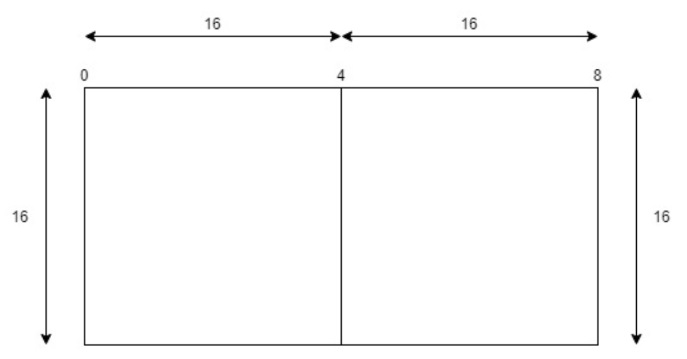
\includegraphics[width=350px, height=175px]{PATTERNMEM.jpg}
\end{figure}\\
Ogni blocco può essere considerato come costituito da $16\times16$ tiles, dove ogni tile non è altro che un agglomerato di pixel. Ogni pixel mantiene un'informazione da 2 bit, e pertanto, poichè ogni tile è $8\times8$ pixel, allora per ogni tile sono necessari 128bit, ossia \emph{16 byte}. Questi 16 byute sono memorizzati tramite i due \emph{bit plane} in cui è decomponibile un tile. Dunque, visualizzando questa tecnica, abbiamo:
\begin{figure}[h]
\centering
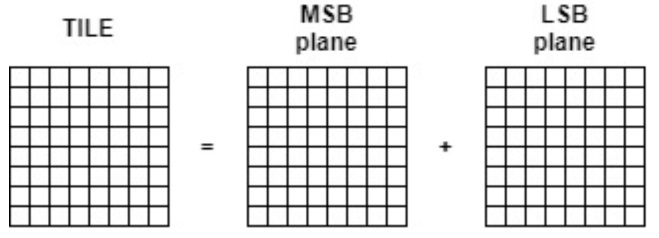
\includegraphics[width=322px, height=116px]{TILE_STORING.jpg}
\end{figure}\\
Il valore contenuto dal pixel ci sarà utile per determinare il suo colore.
\clearpage
\paragraph{Gestione della palette memory}
La palette memory è gestita facendo uso di una piccola porzione dello spazio di indirizzamento della PPU, ossia da $\$3F00$ a $\$3FFF$, con mirroring a partire da $\$3F20$.\\
La palette memory è così organizzata:
\begin{figure}[h]
\centering
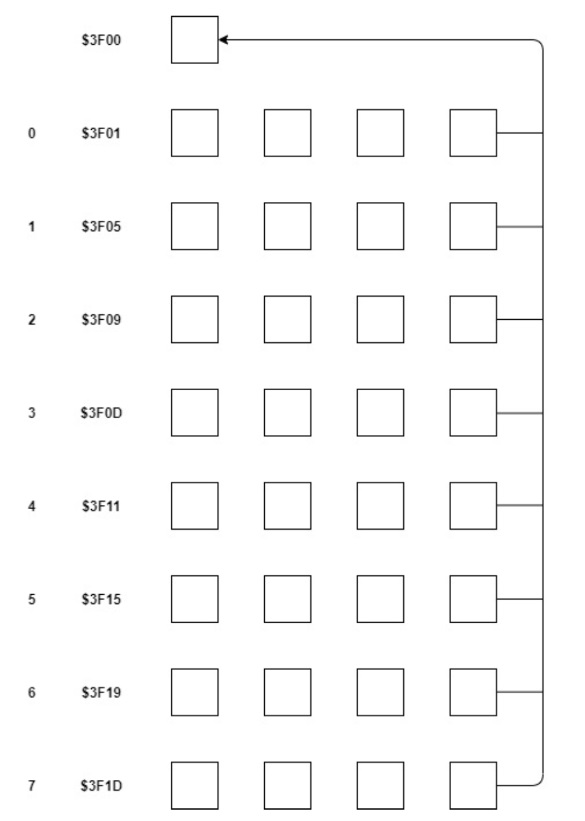
\includegraphics[width=275px, height=400px]{PALETTE_STORING.jpg}
\end{figure}\\
Con quei numeri a fianco delgi indirizzi, si indica l'indice della i-esima palette. Nel contesto della palette, oltre all'indice va specificato anche l'offset, per campionare lo specifico colore della specifica palette. La formula è:
\[
	(PaletteID\cdot 4)+offset=colore
\]
Da notare che per ogni palette c'è un mirroring al colore mantenuto da $\$3F00$, che è il background.

Dunque, concettualmente, il programma \emph{carica} la palette memory, \emph{carica} la pattern memory, e quando la \emph{VRAM} riesce a indirizzare un pixel dalla pattern memory, combinando questa informazione con ciò che è contenuto nell'attributo relativo al pixel, si può ottenere il colore corretto per il pixel da disegnare.
\paragraph{Gestione dello scrolling} Poniamo qui particolare enfasi sulla configurazione grafica della VRAM:
\begin{figure}[h]
\centering
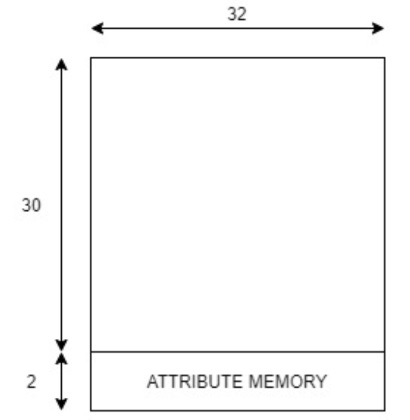
\includegraphics[width=200px, height=215px]{NAMETABLE.jpg}\\
\small\textbf{Nametable}
\end{figure}\\
Spesso i programmi, nel passare da un frame a un altro, cambiano solo lievemente lo scenario, dando l'impressione di star srotolando una bobina (in verticale o in orizzontale). Ciò apre le porte a un meccanism ocomplesso ma fondante della logica di rendering: lo scrolling.
\clearpage
Consideriamo lo scrolling orizzontale:
\begin{figure}[h]
\centering
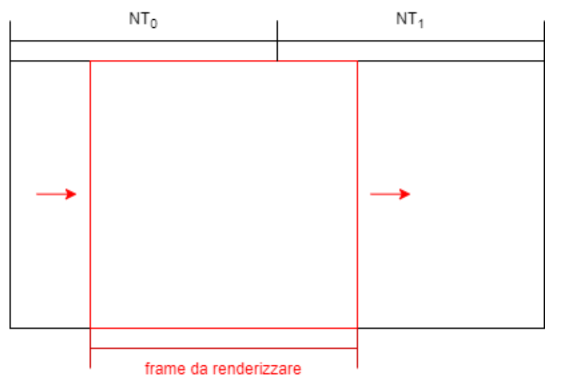
\includegraphics[width=270px, height=190px]{HOR_SCROLL.png}
\end{figure}\\
Il riquadro rossa individua nella fattispecie il frame da renderizzare, che però è posto tra $NT_0$ e $NT_1$. Questa cosa necessita che i tile, o meglio i \emph{pixel}, da renderizzare non devono partire dal punto più estremo in alto a sinistra del singolo nametable, bensì da un offset ben preciso, calcolato a partire dall'angolo estremo in alto a sinistra di uno dei due $NT$.\\
Per calcolare questo offset, prendiamo in esame una granatura per \emph{singolo tile}.\\
La granatura impone di calcolare l'offset con una formula del tipo:
\[
	y\cdot width+ x
\]
È tuttavia facile dimostrare che, scegliendo una stringa da 10 bit, e considerando la prima parte come \emph{coarse y} e la seconda come \emph{corase x}, abbiamo il nostro offset:
\begin{figure}[h]
\centering
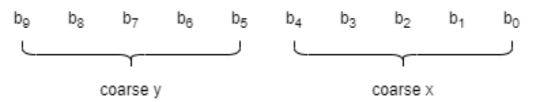
\includegraphics[width=275px, height=50px]{OFFSET_CALC.png}
\end{figure}
Aggiungendo due bit in testa, e arrivando quindi a una stringa di 12 bit totali, possiamo anche individuare qual è il nametable corrente nella fase di rendering.

In realtà, lo scrolling viene svolot con una granatura dell'ordine del pixel, e pertanto necessita che ci siano altre due variabili, nominate \emph{fine x} e \emph{fine y}, che specificano l'offset nel singolo tile.

A questo punto non rimane che legare i tile con i rispettivi attributi. Consideriamo che la attribute memori è grande $64 Byte$. In virtù di ciò, è possibile organizzarla come una matrice di $8\times8$ byte. Ogni byte fa riferimento a una regione di $4\times4$ tiles nella nametable corrispondente di dimensioni $32\times 30$ Bytes. In realtà, è possibile suddividere il singolo byte in quattro regioni da 2 bit ciascuna per poter individuare nella regione quattro sottoregioni da $2\times 2$ tiles. Per ognuna di queste sottoregioni è possibile specificare la palette desiderata, che coprirà quindi un'area pari a $16\times 16=256$ pixel.\\
Due bit sono sufficienti in virtù del fatto che le palettes destinate al rendering del background sono proprio 4 (sono sufficienti dunque solo 2 bit per trarre una delle 4 palette). A questo punto, l'associazione va a 2 a 2 con ogni blocchetto da $2\times 2$ tiles.
\begin{figure}[h]
\centering
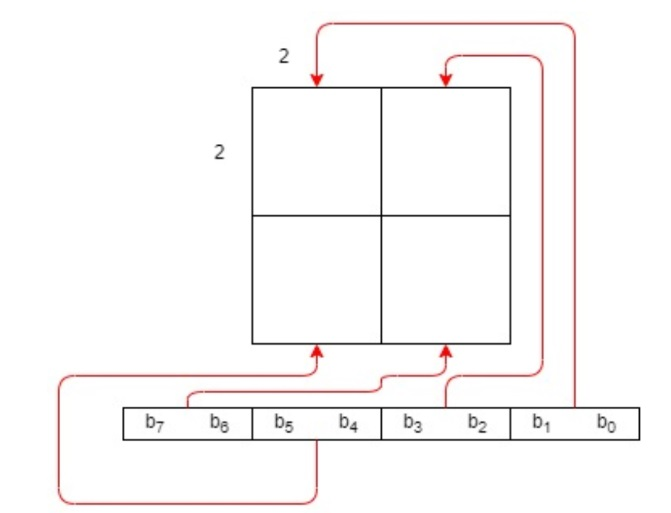
\includegraphics[width=300px, height=255px]{ATT_TILE_MAP.jpg}\\
\small\textbf{Mapping tra Byte dell'attribute memory e le varie regioni da essa rappresentata}
\end{figure}\\
C'è infine da considerare una cosa importante: così come per i tile, va specificato un \emph{attribute offset} per il relativo byte rappresentativo. Tuttavia, per \emph{coarse X} e \emph{coarse Y} sono sufficienti solo 3 bit ciascuno, risparmiano così 4 bit in totale, da poter usare per specificare le palette particolari da utilizzare per la singola regione indirizzata.
\paragraph{Gestione del rendering}
Per poter renderizzare un frame sono utili i cosiddetti \emph{loopy registers}. I loopy register sono dei registri interni alla PPU che consentono la lettura/scrittura della VRAM da parte della CPU, ma anche e soprattutto di supportare il rendering.

I loopyu registers sono i seguenti:
\begin{itemize}
\item{
v: current VRAM (15 bit);
}
\item{
t: temporary VRAM (15 bit);
}
\item{
x: fine X scroll (3 bit);
}
\item{
w: first or second write toggle (1 bit).
}
\end{itemize}
Durante il rendering, la configurazione di t e v è la seguente:
\[
	yyyNNYYYYYXXXXX
\]
dove, a partire dal bit meno significativo, i primi 5 bit indicano l'offset rispetto all'asse orizzontale, i successivi 5 bit l'offset rispetto all'asse verticale, i successivi 2 la nametable scelta, e infine gli altri 3 l'offset rispetto all'asse verticale con granatura interna al tile.

Il punto importante è che, al di là della particolare configurazione di t e v, questi due registri sono influenzati pesantemente dalla comunicazione della CPU con la PPU tramite i vari registri. Ad esempio:
\begin{itemize}
	\item{
		Per una write su $\$2000$ con $d=......BA$, abbiamo:
		\[
			t = ...BA.........
		\]
	}
	\item{
		Per la first write su $\$2005$ con $d=HGFEDCBA$:
		\[
			t = .........HGFED
		\]
		\[
			x = CBA
		\]
		\[
			w = 1
		\]
	}
\end{itemize}
I loopy register vengono settati così, e partecipano attivamente al rendering dei frame.

Quando la PPU esegue, le sue operazioni dipendono dal suo passato. Ad esempio, se la PPU ha eseguito per un certo numero di cicli, allora essa si comporterà in maniera diversa, così come se essa ha eseguito per un certo numero di \emph{scanline}, si comporterà in maniera diversa.

In qualsiasi stato, tuttavia, essa frà uso dei loopy registers, ma non solo: per il rendering si rivelano necessari alcuni shift registers e altre variabili d'appoggio.

Tra gli shift registers ritroviamo:
\begin{itemize}
	\item{
	2 shift-registers di 16 bit ciascuno che memorizzano 2 tile; la parte più significativa contiene i primi 8 pixel da dover renderizzare, mentre la parte meno significativa l'altro tile pre-caricato.
	}
	\item{
	2 shift registers di 8-bit ciascuno che memorizzano gli attributi peri l tile corrente.
	}
\end{itemize}
\clearpage
Gli shift registers si rivelano necessari poichè consentono di renderizzare un pixel alla volta. Concettualmente, quando si avvierà un nuovo ciclo nella parte di rendering grafico, si avrà una disposizione di questo tipo:
\begin{figure}[h]
\hspace*{-1.2cm}
\centering
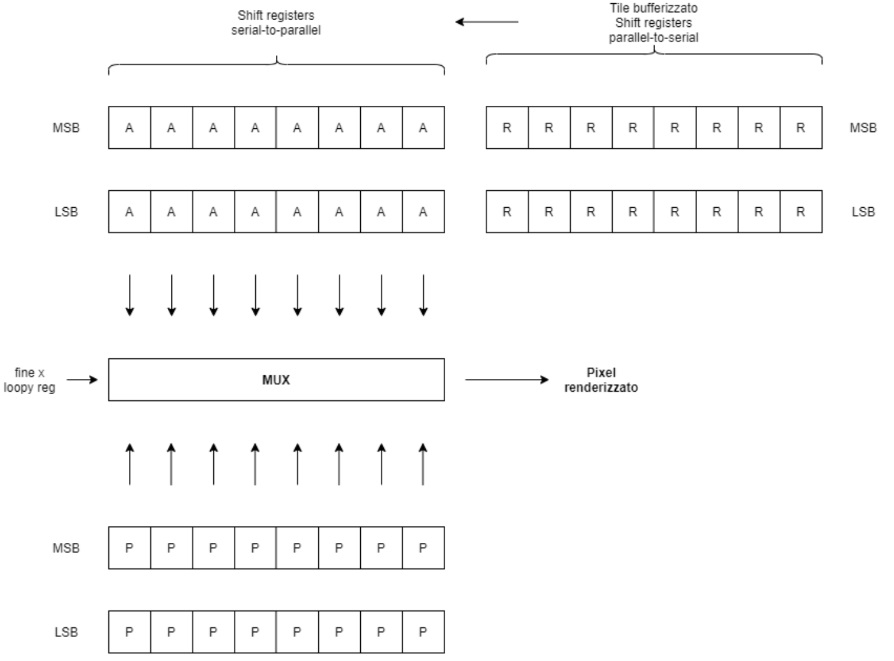
\includegraphics[width=450px, height=330px]{PIXEL_RENDERING_LOGIC.png}
\end{figure}\\
Concettualmente, supponiamo di disporre già una coppia di shift-registers pronti per essere renderizzati. Questi shift-registers sono quelli i cui singoli flip-flop sono etichettati con `A'. Il valore di questi shift-registers si combinano con quelli dei corrispondenti attributi (shift-registers i cui singoli flip-flop sono etichettati con `P'), secondo il valore specificato dal loopy register \emph{fine x}: il multiplexer consente di selezionare il pixel da renderizzare avendo come segnale di abilitazione \emph{fine x}. 

Ovviamente quanto appena descritto fa riferimento alla situazione nominale per cui si dispone di tutti gli shift-registers riempiti, tuttavia la logica di controllo è più complessa di così; difatti si spenderanno cicli di clock della PPU a caricare i dati da immettere negli shift-registers, ad aggiornare la VRAM, ecc.
\section{Analisi dei requisiti}
\subsection{Prima iterazione}

\subsection{Seconda iterazione}

\subsection{Terza iterazione}

\section{Design funzionale/non-funzionale}
\subsection{Prima iterazione}

\subsection{Seconda iterazione}

\subsection{Terza iterazione}

\section{Prospettiva implementativa}
\subsection{Prima iterazione}

\subsection{Seconda iterazione}

\subsection{Terza iterazione}








\end{document}